\documentclass[12pt]{article}

\author{Scott Kenning}
\title{A Photonic Optimization Package}


\usepackage{tcolorbox}
\usepackage{siunitx}
\tcbuselibrary{minted,breakable,xparse,skins}

\definecolor{bg}{gray}{0.95}
\DeclareTCBListing{mintedbox}{O{}m!O{}}{%
  breakable=true,
  listing engine=minted,
  listing only,
  minted language=#2,
  minted style=default,
  minted options={%
    linenos,
    gobble=0,
    breaklines=true,
    breakafter=,,
    fontsize=\small,
    numbersep=8pt,
    #1},
  boxsep=0pt,
  left skip=0pt,
  right skip=0pt,
  left=25pt,
  right=0pt,
  top=3pt,
  bottom=3pt,
  arc=5pt,
  leftrule=0pt,
  rightrule=0pt,
  bottomrule=2pt,
  toprule=2pt,
  colback=bg,
  colframe=orange!70,
  enhanced,
  overlay={%
    \begin{tcbclipinterior}
    \fill[orange!20!white] (frame.south west) rectangle ([xshift=20pt]frame.north west);
    \end{tcbclipinterior}},
  #3}

\begin{document}

\maketitle

\section{Introduction}

\subsection{Motivation}
Photonic design often takes place by using analytic principles to guide simulations and subsequent manufacturing runs to test devices. This process works well, but there are several reoccurring themes during the design process.
\begin{enumerate}
\item Convergence testing must be often performed to ensure simulation results are accurate.\label{list.convergence}
\item Optimization of structures (beyond the realm available with analytic math) is often carried out through brute force means (i.e., parameter sweeps).\label{list.opt}
\item It is cumbersome to draw structures in simulation software when models in well-developed layout tools already exist.\label{list.drawing}
\item Simulation scripts are often ``quick and dirty", meaning they lack readability and structure. Often times, they are copy-and-pastes of previous problems modified slightly.\label{list.structure}
\end{enumerate}
We seek to address these issues through the design of a Python package that carries out tasks relevant to solving the above issues. The vision for the Python package was shaped through interaction with photonic designers and firsthand experience working on photonic design problems. 

\subsection{Goals}
The goals of this project are separated off based on the classification of them being a ``process" problem or a ``design" problem. Process problems refer to \ref{list.convergence}, \ref{list.drawing}, and \ref{list.structure} in the above motivation list, while design problems relate to the generation of a flexible optimization framework related to item \ref{list.opt}.

\subsubsection{Process Problems}
These goals relate to generating useful code that abstracts the idea of a ``simulation". This relates to breaking the problem into a few key components that are often universal across photonic simulations.
\begin{itemize}
\item One-time initialization routines: These routines often initialize the underlying simulation engine. They often are called once in the beginning of a script running. 
\item Loading desired simulation parameters: Photonic simulations often involve designing devices with an assorted variety of parameters. 
\item Drawing: Structures in a photonic simulation must be drawn once per iteration. In a single script, the structures may be changed (e.g., during design parameter sweeping).
\item Running: After structures are drawn, some sort of simulation must take place.
\item Post-processing: This may involve exporting fields, generating images of results, performing calculations, etc.
\end{itemize}

\subsubsection{Design Problems}
Built on the back of the above process problems are design problems. Here, we are concerned with efficiently running simulations that yield optimized photonic devices. This is a difficult concept to address, and we will therefore outline a few goals.
\begin{itemize}
\item Allow users to run optimization algorithms on design parameters.
\item Allow for specialized tools like adjoint methods to be used for gradient calculations in optimization problems.
\end{itemize}

\section{Addressing Process Problems}
Before ``Design Problems" are addressed, it is important to solve the ``Process Problems". By addressing them in this order, it is possible to fit an optimization framework cohesively inside.

There are two standards for scientific computing that we will allow usage of with our code: MPI and HDF5. Ultimately, usage of MPI is at the mercy of the backend simulation software (Lumerical and MEEP \cite{meep} both support it, for example). Since this project provides wrapper functionality around an arbitrary software suite, we do not want it to interfere with MPI and cause deadlocking. Roughly speaking, this translates into all processes call identical backend simulation calls. To do this, we will define methods in the following section that allow MPI-interfacing software to be called within. 

HDF5 is a standard file type that allows storage of large amounts of data in typically an array format. It is widely used and accessible. It is attractive for several reasons.
\begin{itemize}
\item Metadata may be easily stored alongside simulation results. This is useful for record keeping and knowing exactly what simulation parameters were used for a given dataset. 
\item It is compressed and in a binary format (it is more compact then other data formats).
\item It is easily compatible with Python, Matlab, MEEP, Lumerical, etc. Newer .mat files are actually based off of it.
\end{itemize}
This standardized file format will be widely used in the software.

\subsection{The Simulation Class}
To address process problems, we propose the \mintinline{latex}{Simulation} class. Although the exposed user-interface is rather simple, it provides behind-the-scenes machinery to ensure ease of use and fault-tolerant behavior. The user interface is previewed below. 
\begin{mintedbox}{python}
class Simulation:
	def __init__(self, logname : str, working_dir : str, catch_errors=True):     
	    ...

    def draw(self, parameters : dict[str, typing.Any]) -> None:
        pass
    
    def run(self, parameters : dict[str, typing.Any]) -> Result:
        return Result(parameters)
    
    def process(self, result : Result, parameters : dict[str, typing.Any]) -> Result:
        return result
        
    def oneOff(self, iteration_parameters: dict[str, typing.Any], iteration=1, total_iterations=1) -> typing.Union[Result, None]:
    	...
        
    def basicSweep(self, parameters: dict[str, list[typing.Any]]):
    	...
\end{mintedbox}
All commands to an MPI-dependent backend should be placed within \mintinline{latex}{draw}, \mintinline{latex}{run}, and \mintinline{latex}{process}.  

\subsubsection{Running Basic Parameter Sweeps}
A task that often comes up is running parameter sweeps. This is done by using \mintinline{latex}{Simulation.basicSweep}. The block diagram of this helper function is shown in Figure \ref{fig.basic_sweep_blocks}.
\begin{figure}
\centering{
\includegraphics[width=\textwidth]{figs/basic_sweep_blocks.png}
}
\caption{The block diagram of \mintinline{latex}{Simulation.basicSweep}. Red lines indicate error handling routes and the black represent normal program flow in the absence of errors.}
\label{fig.basic_sweep_blocks}
\end{figure}
The goal of this routine is to provide fault-tolerant running of many simulations. For example, a list of simulations (their parameters) can be loaded from a CSV file using the \mintinline{latex}{CSVParameterLoader} class and passed directly to the \mintinline{latex}{basicSweep} function. If at any point in the \mintinline{latex}{draw}, \mintinline{latex}{run}, or \mintinline{latex}{process} routines an exception is raised, the machinery will salvage as much as possible and then continue running other simulations. Ample logging allows the resulting suppressed exceptions to be debugged by the user. 

To actually write a simulation, the user inherits from the \mintinline{latex}{Simulation} class and overrides atleast \mintinline{latex}{draw} and \mintinline{latex}{run}. Overriding \mintinline{latex}{process} is optional. The \mintinline{latex}{process} routine ultimately gives the user freedom to add additional data to the results of the \mintinline{latex}{run} routine.

\subsubsection{Running a One-Off Simulation}
The \mintinline{latex}{oneOff} function actually provides the same functionality as \mintinline{latex}{basicSweep}, but for the case where there is only a single set of parameters. In fact \mintinline{latex}{oneOff} is actually just called many times by \mintinline{latex}{basicSweep} and implements the exception handling logic.

\subsection{The Result Class}
To continue addressing process problems, we propose the \mintinline{latex}{Result} class. Arguably simpler than the \mintinline{latex}{Simulation} class, it has one purpose: save desired results and their associated metadata. 

\begin{mintedbox}{python}
class Result:
	def __init__(self, parameters: dict[str, typing.Any], **values): 
	    ...
\end{mintedbox}

This is just achieved by returning a \mintinline{latex}{Result} object from the \mintinline{latex}{run} or \mintinline{latex}{process} routines of the \mintinline{latex}{Simulation} class. The constructor's signature is above, and is the only relevant function for the end user. 

The \mintinline{latex}{parameters} variable needs to be a Python \mintinline{latex}{dict} that specifies metadata to be saved. For example, and as shown in Figure \ref{fig.result_metadata}, design parameters for a particular device are stored as metadata. The actual folder name in the HDF5 file is generated randomly and uniquely, so the metadata is the differentiation feature of each folder of data in the simulation result files.

\begin{figure}
\centering{
\includegraphics[width=\textwidth]{figs/result_metadata.png}
}
\caption{A screenshot of the resulting HDF5 file displayed in ViTables after many simulations were ran. The blue folder icons indicate HDF5 groups, which have the simulation parameters used saved in their metadata. Additional data (which is not metadata) was saved inside each group (e.g., \mintinline{latex}{dJ_db}).}
\label{fig.result_metadata}
\end{figure}

To save data that is not metadata (e.g., field quantities), they are simply passed in as \mintinline{latex}{kwargs} to the constructor of \mintinline{latex}{Result} as shown by example below.
\begin{mintedbox}{python}
	...some simulation code...
	return Result(parameters, f0=f0, dJ_du=dJ_du, dJ_db=dJ_db, min_db=np.asarray(min_db), all_du_db=all_du_db, wavelengths=self.wavelengths)
\end{mintedbox}

For example, passing \mintinline{latex}{f0=f0} means ``save the variable in the above simulation code (right hand side of equal sign) as a variable named \mintinline{latex}{f0} (left hand side of equal sign) in the HDF5 file". Since there is often no need to change the name of the variable used in the script to something else in the HDF5 file, often times both sides of the equal sign will have the same variable name, leading to a notation that might look strange.

The \mintinline{latex}{Result} class can handle data types that HDF5 supports. This includes most of the \mintinline{latex}{numpy} array types.

\subsection{The ConvergenceTest Class}
The \mintinline{latex}{ConvergenceTest} class performs exactly what it sounds like: convergence testing. Ultimately, the user guesses at what range of parameters needs to be swept. In addition, convergence criteria is supplied. It can optionally generate plots that would provide proof of convergence, and will return the suggested parameters required for appropriate convergence. See the in-code documentation for more information found in \mintinline{latex}{pdt/core/Simulation.py}.

\section{Addressing Design Problems}
Addressing design problems, which are essentially in the form of optimization problems, is quite nuanced depending on what solver is used. In FDTD, it is possible to efficiently obtain gradient information of a design with two simulations. There are two strategies available that fall under ``adjoint methods", and usually one is implemented to a degree by the solver. In the case of MEEP, ``density-based" methods are employed. 

\subsection{The DesignRegion and MaterialFunction Classes}

Density-based methods are often used to design structures that are completely arbitrary. That is, as many degrees of freedom as possible are given to the optimization code. This often results in a grid with hundreds of ``pixels" being changed around. This software has tools (such as \mintinline{latex}{DesignRegion} and \mintinline{latex}{MaterialFunction}) that are useful for designing ``traditional" structures like tapers, mode converters, etc. It ultimately back-propagates the derivative given by the density methods (for each material pixel) to the design parameters. However, this is beyond the scope of this high-level document. These features are best explained by the examples in \mintinline{latex}{pdt/designs/} or the Pydocs in the code.

\subsubsection{Design Perturbation}
Since any design that is optimized is likely projected onto a discrete grid, perturbing the design is not guaranteed to actually change the design once it is ultimately placed on the discrete simulation grid. Therefore, this software collects information about that grid and calculates the perturbation of each design parameter required to allow the simulator to see a unique design.

\begin{figure}
\centering{
\includegraphics[width=0.85\textwidth]{figs/toy_taper_example.png}
}
\caption{A simple taper example. We naively assume that we can simply connect two waveguides, and see if the computer can come up with something better in the dashed region.}
\label{fig.toy_taper_example}
\end{figure}

Consider the design of a simple taper, as shown in Figure \ref{fig.toy_taper_example}. We assume no knowledge of taper design, and naively assume that the two waveguides can simply be connected together. We wish for the computer to optimize the waveguide width in the dashed box to maximize power transmission from the fundamental mode in one waveguide to the other. This is actually an example in \mintinline{latex}{pdt/designs/}, so we will briefly examine the relevant sections of it. 

To parameterize the design with respect to some degrees of freedom, we represent the width of the designed section along the horizontal direction with a weighted summation of Legendre polynomials up to a certain order. In effect, the computer can wiggle the boundaries around. If it modifies the weight of the linear Legendre polynomial, the yellow pixels in Figure \ref{fig.design_perturbation} will then be shaded in, as shown. 

\begin{figure}
\centering{
\includegraphics[width=0.4\textwidth]{figs/design_perturbation.png}
}
\caption{If the weight associated with the linear Legendre polynomial is marginally increased, the pixels of material in yellow will be changed. Note that this figure is what would occur if the design in Figure \ref{fig.toy_taper_example} is changed. In reality, the perturbation will be made as small as possible, so long as the underlying discrete grid of material is actually changed.}
\label{fig.design_perturbation}
\end{figure}

\subsubsection{Sensitivity Information and Gradient Back-Propagation}\label{sec.adjoint}
Density-based adjoint solvers like MEEP return ``sensitivity information" \cite{meep_adjoint}. This information describes how, if pixel $j$ of material changes, the figure of merit changes (e.g., the transmission of power through a structure). If we consider the design in Figure \ref{fig.toy_taper_example}, a solver like MEEP would return data that is visualized by Figure \ref{fig.sensitivity_information}. Combined with information from Figure \ref{fig.design_perturbation}, we can compute the gradient with respect to the design parameters (in this case, the coefficients to the polynomials generating the taper width).

Figure \ref{fig.design_perturbation} gives us $\frac{\partial \epsilon_j}{\partial b_i}$, while Figure \ref{fig.sensitivity_information} gives us $\frac{\partial f}{\partial \epsilon_j}$. $f$ represents our figure of merit, $\epsilon_j$ represents the dielectric constant at a pixel indexed by $j$, and $b_i$ represents a design parameter indexed by $i$. Through the chain rule, we can compute $\frac{\partial f}{\partial b_i}$.
\begin{equation}
\frac{\partial f}{\partial b_i} = \sum_j \frac{\partial f}{\partial \epsilon_j} \frac{\partial \epsilon_j}{\partial b_i}
\end{equation}

This computation of the gradient from sensitivity information and perturbation of design parameters is one of the key purposes of the classes described in this section.

\begin{figure}
\centering{
\includegraphics[width=0.4\textwidth]{figs/sensitivity_information.png}
}
\caption{At yellow colors, an increase in the dielectric constant would increase transmission. At purple colors, a increase in the dielectric constant would decrease transmission.}
\label{fig.sensitivity_information}
\end{figure}

\subsection{The ScipyGradientOptimizer Class}
This class wraps optimization function calls in a way that is compatible with the \mintinline{latex}{Simulation} and \mintinline{latex}{Result} class. Detailed documentation can be found in the Pydocs, but a brief outline of the important features that address design problems are presented here.

The key takeaway is that this class provides a single interface for performing optimization that seamlessly allows for computation of the gradient using first-difference or custom means.

\subsubsection{First-Difference Gradient Calculation}
This class is capable of using first-difference methods to compute the gradient, which will then be fed to a generic optimization algorithm. If there are $N$ degrees of freedom in the design, $N+1$ simulations are required. There are more efficient ways to obtain this gradient information, but the first-difference method is a nice way to debug.

Each design parameter is perturbed by an amount prescribed by the \mintinline{latex}{DesignRegion} and \mintinline{latex}{MaterialFunction}. Then the figure of merit is extracted from the \mintinline{latex}{Result} class to perform the first-difference calculation.

\subsubsection{Custom Gradient Calculation}
The user may have their own solver-specific method of computing the gradient. In the examples provided in \mintinline{latex}{pdt/designs/}, this is in the form of utilizing the adjoint solver in MEEP to provide sensitivity information. The \mintinline{latex}{DesignRegion} and \mintinline{latex}{MaterialFunction} classes can be used to compute the gradient as outlined in Section \ref{sec.adjoint}. This is then returned by the user in a \mintinline{latex}{Result} object. \mintinline{latex}{ScipyGradientOptimizer} will then utilize that information if the name of the field inside the \mintinline{latex}{Result} containing the gradient is provided. Otherwise, \mintinline{latex}{ScipyGradientOptimizer} will default to first-difference methods.

The importance of ``custom gradient calculation" methods is that in electromanetics, adjoint methods can be used. Regardless of the number of design variables to optimize, only two simulations are required to obtain the information necessary.

\subsection{Example Results: Waveguide Taper}
A waveguide taper presents an interesting toy example: give the optimization script a poor initial state (depicted in Figure \ref{fig.toy_taper_example}) and see if it comes up with a better design. The code for this example is found in \mintinline{latex}{pdt/designs/} and is named \mintinline{latex}{WaveguideTaperAdjvsFD.py}.

The device being designed transfers light from a \SI{400}{\nano\meter} waveguide into a \SI{1}{\micro\meter} waveguide. The allowed taper length is \SI{1}{\micro\meter}, which makes it incredibly aggressive. The first ten Legendre polynomials are used in the construction of the taper width along the propagation direction.

The initial device has $\left|S_{11}\right|^2 \approx 0.82$, averaged across three wavelengths (\SI{1.50}{\micro\meter}, \SI{1.55}{\micro\meter}, and \SI{1.60}{\micro\meter}). The final optimized device has $\left|S_{11}\right|^2 \approx 0.98$. A cartoon of the final device is found in Figure \ref{fig.toy_taper_example_optimized}. This software generates GIF renders of the optimization process for fun, and the one for this example can be found in \mintinline{latex}{pdt/designs/renders/}.

\begin{figure}
\centering{
\includegraphics[width=0.8\textwidth]{figs/toy_taper_example_optimized.png}
}
\caption{The final optimized state of the taper.}
\label{fig.toy_taper_example_optimized}
\end{figure}

\subsection{Example Results: Strip-to-slot Mode Converter}
We adapt a device from \cite{deng} to incorporate a stripload. The original device as outlined in \cite{deng} does not incorporate striploading, which is necessary if the resulting slot waveguide will be used in modulator designs. In effect, we add the blue regions into the slot section of the device, depicted in Figures \ref{fig.slot_xs} and \ref{fig.s2s_striploading}.

\begin{figure}
\centering{
\includegraphics[width=0.4\textwidth]{figs/s2s_striploading.png}
}
\caption{A modified design based off of the work of \cite{deng}. This is actually the optimized design.}
\label{fig.s2s_striploading}
\end{figure}

\begin{figure}
\centering{
\includegraphics[width=0.4\textwidth]{figs/slot_xs.png}
}
\caption{The cross section of a striploaded slot waveguide. This is a cross section of the far right side of Figure \ref{fig.s2s_striploading}.}
\label{fig.slot_xs}
\end{figure}

The optimizer was given the opportunity to wiggle around the green taper boundaries and the blue stripload boundaries. Figure \ref{fig.s2s_striploading} is a cartoon of what was designed by the program. It transmits roughly $97\%$ of power in the fundamental mode of the strip waveguide to the slot waveguide. This is on-par with the claims made by \cite{deng}. Note that the simulation was 2D, and the index of the silicon ridge was calculated using rough averaging techniques. 

\section{Conclusion}
This software provides an interface to structure simulation code around that addresses the ``process problems". The \mintinline{latex}{Simulation} class provides general logging facilities, error logging (and suppression, if desired), standardized functions to override for code clarity, and organization of results. Alongside the \mintinline{latex}{Result} class, its functionality is extended to saving simulation metadata and data generated in a standardized manner. 

In addition, a simple interface is provided for optimization that wraps around the \mintinline{latex}{Simulation} and \mintinline{latex}{Result} classes. It offers generic first-difference gradient calculations and leaves room for using solver-specific adjoint information. Through this process, it abstracts away challenges including making sure a perturbational change in the design variables actually results in the discrete material grid used by the solver changing. It greatly facilitates optimization problems in FDTD simulations.

Examples have been provided in \mintinline{latex}{pdt/designs/}. A taper example was discussed in this document, but a more sophisticated example such as the design of a strip-to-slot mode converter \cite{deng} is also available. These examples are 2D structures (they easily run on most computers), but there is nothing preventing the extension to 3D.

\newpage
\bibliographystyle{IEEEtran}
\bibliography{project_report.bib}


\end{document}